\section{Solving differential equations by series expansion}
\label{sec:series}
The solution of a system of linear differential equations by series
expansions is well known in the mathematical literature.
The analytic continuation of the solution of a differential equation,
from its initial region of convergence to an external arbitrary point
is the topic that we want to discuss, applied to the specific case of
Feynman integrals.
In this Section we present some basic definitions
to set the stage of our discussion.


\subsection{An introductory example}
\label{sec:example}
The method can be illustrated with a simple example.
Let us consider the differential equation
\be
\left\{
\begin{array}{l}
f'(x) +\frac{1}{2x (1+x)}f(x)=\frac{1-2x}{8x (1+x)}\\
f(0)=\frac14 
\end{array}
\right.
\label{eq:exampleeqdiff}
\ee
with $x$ a real variable.
We introduce $f(x)=x^r \sum_{k=0}^\infty c_k x^k$,
as an expansion around $x=0$,
with $c_k$ arbitrary coefficients.
We replace $f(x)$ with the power series in the
associated homogeneous differential equation,
we collect all the terms with the same power of $x$ and
obtain an infinite set of algebraic equations in the unknowns $c_k$.
One of the equations,
associated to the lowest power of $x$ and called indicial equation,
assigns the value of the exponent $r$,
which in this example turns out to be $r=-1/2$,
while the other relations determine all the $c_k$ but one;
we choose arbitrarily the latter, and set e.g. $c_0=1$.
We eventually obtain
\be
f_{hom}(x)=\frac{1}{\sqrt{x}}\left(
1+\frac12 x -\frac18 x^2 + \frac{1}{16} x^3+...
\right)
\ee
A particular solution is obtained by applying
the variation of the constant method,
where the inverse of the homogeneous solution,
multiplied by the inhomogeneous term,
is expanded about $x=0$ and easily integrated
\be
f_{part}(x)=
f_{hom}(x)
\int_0^x dz\, \frac{1-2 z}{8 z (1+z)}\, f^{-1}_{hom}(z)
=
\frac14 -\frac16 x+ \frac{1}{15 x^2}- \frac{4}{105} x^3+...
\label{eq:ex1}
\ee
The general solution is given by $f(x)=f_{part}(x)+C f_{hom}(x)$.
In order to satisfy the boundary condition $f(0)=1/4$ we set $C=0$.

The solution eq.~\ref{eq:ex1} is valid in the proximity of $x=0$,
with a convergence radius of 1,
determined by the presence of a singularity at $x=-1$.
The latter can be already read from the homogeneous equation,
with the $1+x$ factor in the denominator.
The regularity of the solution at $x=0$ is enforced by the boundary condition,
which effectively discards the homogeneous solution,
with its singular $1/\sqrt{x}$ behaviour.
Also the latter could be read from the homogeneous equation,
from the $2x$ factor in the denominator.

%%%%%%%%%%%%%%%%%%%%%%%%%%%%%%%%%%%%%%%%%%%%
\subsection{Singularities and branch cuts}
\label{sec:cuts}
We consider now the same first-order linear differential equation
presented in eq.~\ref{eq:exampleeqdiff},
now as a function of a complex variable $z$.
The series representation obtained in eq.\ref{eq:ex1}, replacing $x\to z$,
converges in the complex plane $z$ inside a disc $\Gamma_0$
centered around the boundary condition point $z_0=0$.
We can analytically continue the solution into a new disc $\Gamma_1$,
centered at a point $z_1$ internal to $\Gamma_0$,
provided that $\Gamma_1$ does not include
any singular point, in our example of $z=-1$,
as illustrated in Figure \ref{fig:analcont} by the blue and red circles.
It is possible to demonstrate that this procedure is unique.
\begin{figure}
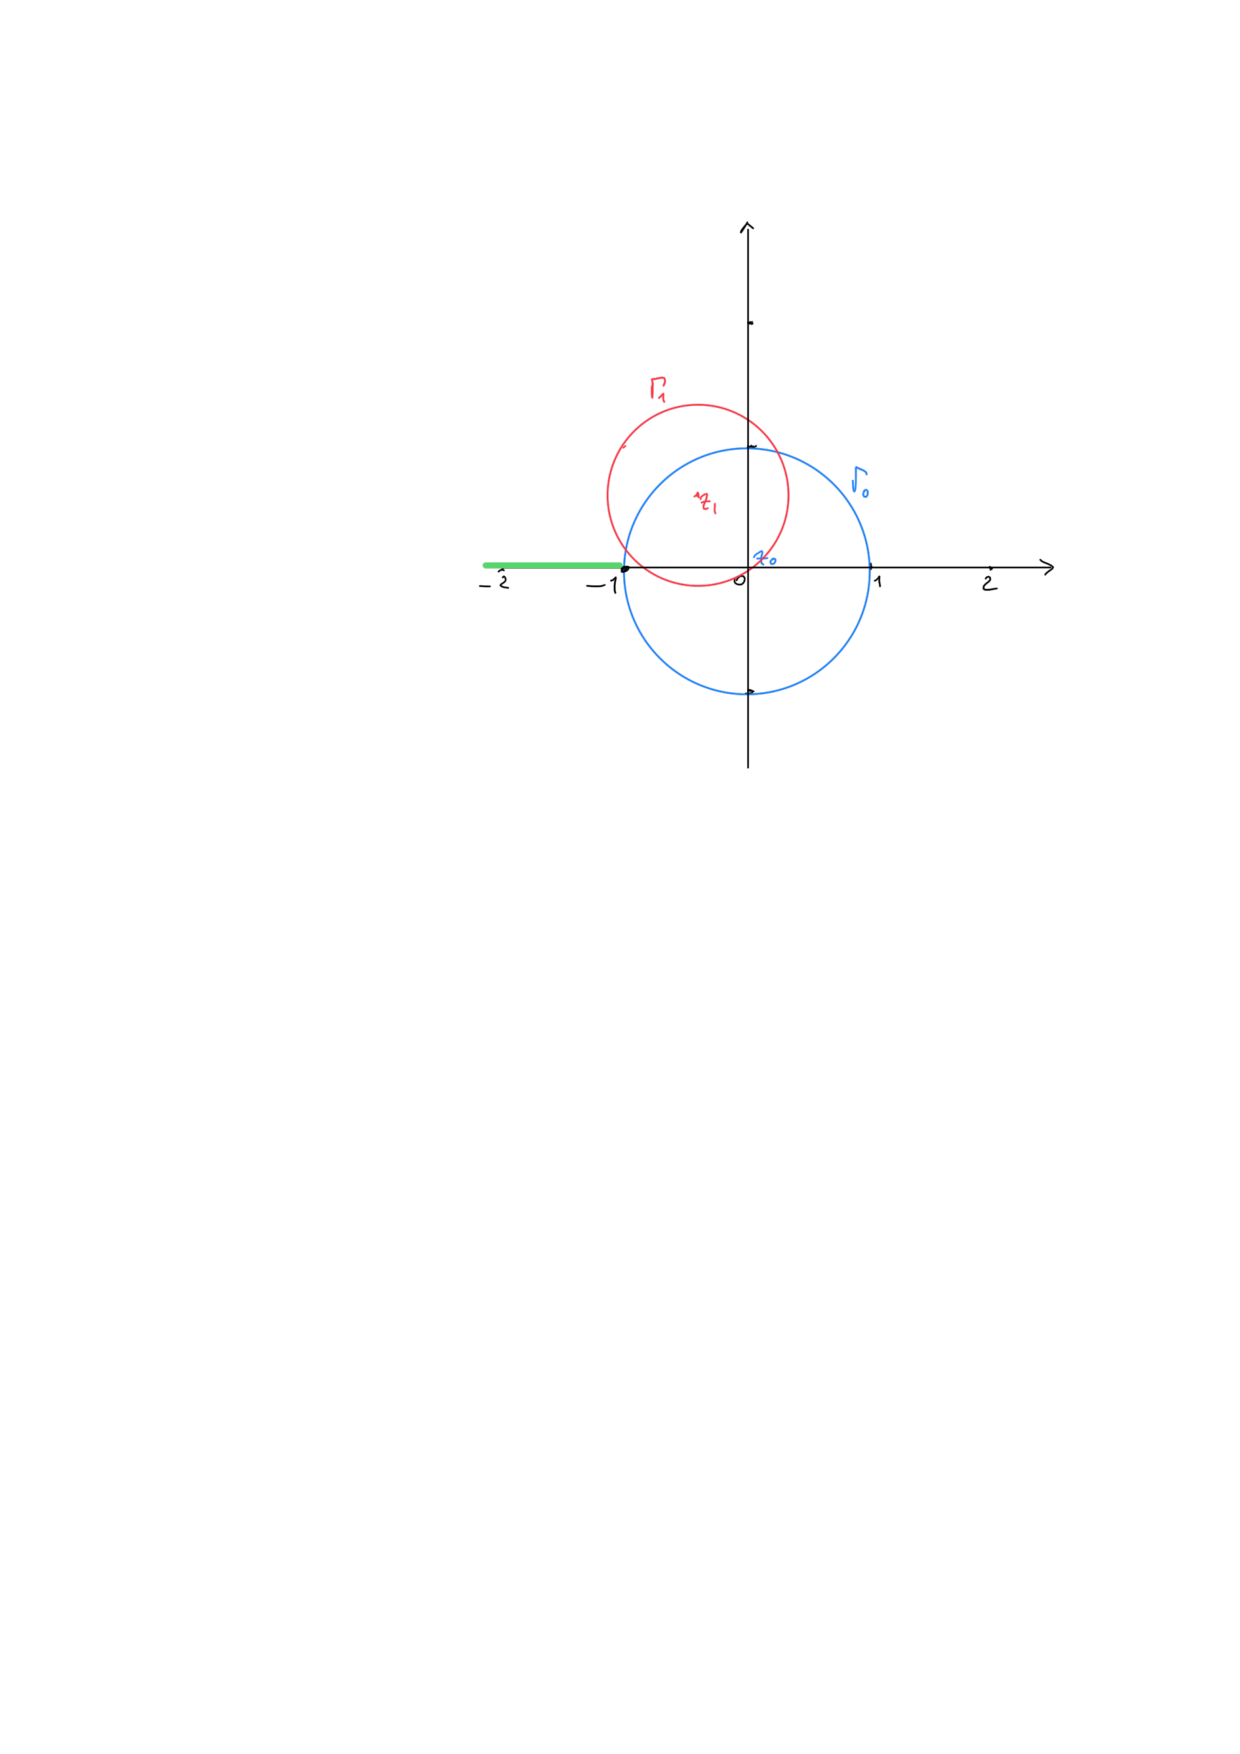
\includegraphics[scale=0.65]{continuazione-analitica.pdf}
\caption{\label{fig:analcont}
  Example of analytic continuation}
\end{figure}

The presence of singularities in the homogeneous or also in the inhomegeneous
coefficients of the differential equation
requires a careful definition of the analytic continuation.
In the frequent physical case of simple poles in the homogeneous coefficient,
we obtain a logarithmic behaviour of the solution.
The latter can be made single-valued
by adding cuts in the complex plane,
so that we specify the Riemann sheet where we evaluate the function.
This feature is clearly not present in the power series representation,
but must be introduced to allow for a physical interpretation of the results.


A simple algorithm to assign the cuts can be devised by noticing that
we can group all possible singular points with respect to $z$
in two categories,
those lying on the $z$ real axis and those with a non-vanishing imaginary part.
$i)$ We collect all the singularities on the real axis,
we identify the rightmost one and we cut from that point to $-\infty$.
$ii)$ For a singular point located at $c$ in the complex plane,
we cut parallel to the imaginary axis
from $c$ upwards to $(\mathrm{Re}(c),+i \infty)$ if $\mathrm{Im}(c)>0$ and
downwards from $c$ to $(\mathrm{Re}(c),-i \infty)$ if $\mathrm{Im}(c)<0$.
An illustration is given in Figure \ref{fig:freestrip} by the green lines,
assuming that
$z=-1,-3/2,-1+i,-1-i,1/2+i/4,1/2-i/4$ are singular points and that
there are no other singularities on the real axis for $\mathrm{Re}(z)>-1$.
This procedure leaves a simply connected Riemann surface,
because all the cuts are applied ``outwards'' and never intersect each other.
\begin{figure}
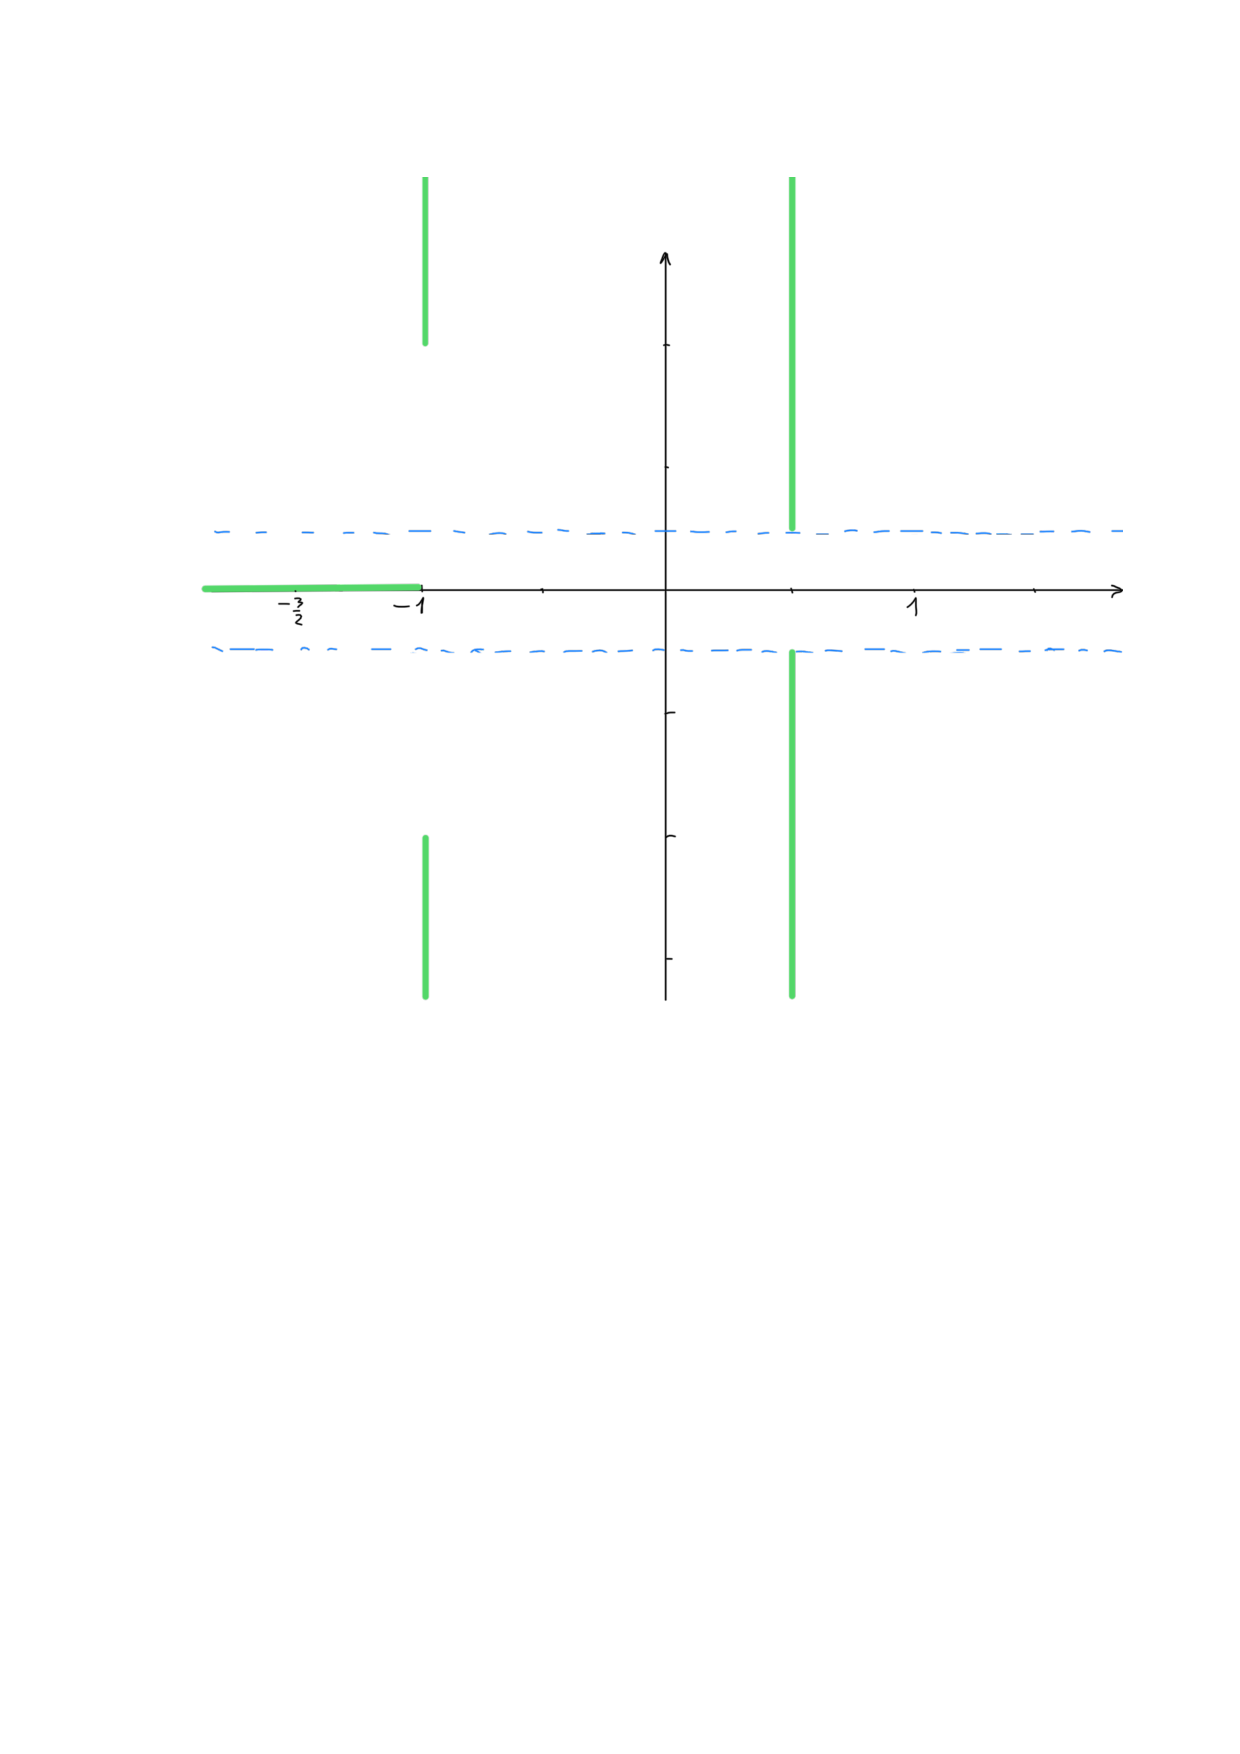
\includegraphics[scale=0.45]{free-strip-ok.pdf}
\caption{\label{fig:freestrip}
  Example of cuts assignment.}
\end{figure}
Given a solution for the unknown function $f(z)$ olomorphic inside a disc
$\Gamma_0$,
the uniqueness of the analytic continuation 
and the simply connected topology of the domain
make the solution single-valued in the whole domain.
In Figure \ref{fig:freestrip} we illustrate the above example
drawing in green the cuts.
In dashed-blue we highlight the presence of a strip of the $z$ complex plane,
which is by construction free of singularities
and will turn out to be central in the implementation of the algorithm:
it is defined by looking for the complex-valued singular point
with the smallest (in absolute value) imaginary part;
the latter defines the width of the strip,
which spans the whole plane, parallel to the real axis.


A choice for the cuts on the real $z$ axis different\footnote{
  We can e.g. choose to put some of the cuts from the singular point to
  $+\infty$, yielding a different inequivalent Riemann surface.
  }
than the one described in $i)$
can lead to a different determination of the solution.
This ambiguity can be discussed and solved,
in the light of the Feynman prescription for the particle propagators,
which enforces the causality requirement of the theory.
If we consider, for the sake of simplicity,
the propagator $\Pi(s)=i/(s-m^2+i\varepsilon)$ of a massive scalar field,
we see that the kinematic invariant $s$ is real,
but the Feynman prescription shifts it indeed to $s+i\varepsilon$
in the upper half of the complex $s$ plane.
We adopt the same prescription for the kinematic variables
of the differential equation,
which implies that
the complete evolution of the solution from the BCs to the point of interest
is performed not on the real axis,
but in the complex plane of the kinematic variable,
and, more precisely, in one specific half of that complex plane.
Having a prescription which pushes the solution of the differential equation
in one specific half of the $z$ complex plane,
we implicitly choose the determination of the solution compatible
with the BCs.
The remark that we study the solution in the whole complex plane
sets in a natural way the framework to handle Feynman integrals
with internal complex masses.


\subsection{Evaluating the solution for arbitrary values of its arguments}
\label{sec:continuation}
The discussion of
the analytical continuation of a function of several variables
can be a tremendous challenge and
we find it convenient to discuss one variable at a time,
while keeping all the others constant with a given numerical value.
With this choice,
all the singular points with respect to the kinematic variable under discussion
are uniquely identifed and are constant.

The solution is conveniently expressed in terms of adimensional variables,
which can be obtained by rescaling the kinematic variables with a dimensional
constant, typically a mass.
We discuss first the case by a real-valued mass.
We define $x=(s+i\varepsilon)/m^2$,
and we remark that dividing by a positive real number clearly does not change
the sign of the infinitesimal imaginary part of the Feynman prescription.
In this case, we find two sets of potential singularities,
depending whether the points are real- or complex-valued.
The former are typically associated with physical (pseudo-)thresholds,
while the latter often appear in the linearisation
of square root factors in the differential equations.


Following this distinction,
we introduce cuts in the complex plane,
as anticipated in Section \ref{sec:cuts}.
%one cut goes from the rightmost real-valued singularity to $-\infty$;
%for the complex-valued singularities, we take vertical cuts,
%as illustrated in Figure \ref{fig:freestrip}.
When moving from one point to another of the kinematic variable,
we can always choose a path inside the strip free of singular points,
where we can compute,
step by step, a convergent Taylor expansion of the solution.\\

The nice example with the colored circles.\\

We consider now the rescaling of the kinematic invariants by a complex mass,
which induces a small deformation of the setup described above
in the real-mass case.
We define $z=s/\mu^2$
by dividing the kinematic invariant $s$ by a complex mass squared $\mu^2$,
with $\mu^2=m^2-i\Gamma m$
where $m$ and $\Gamma$ are the pole values of the propagator.
The variable $z$ will obviously be complex valued,
and we observe the consistency between
the sign of the imaginary part of the Feynman prescription
and the sign of the imaginary part of this adimensional complex variable.
All the singular points are shifted.
Those which are complex valued simply change their position, while
the ones on the real axis acquire an imaginary part.
The single cut on the real axis is now replaced by one horizontal cut for each
singular point, each with its imaginary part.
Provided that we choose a path that avoids the intersection with all these
horizontal cuts, we can still draw a path,
inside the singularity-free strip,
connecting any two points associated to two values of the kinematic variable.\\

Illustration of the cut position with complex masses.\\

We conclude that we can always draw,
with either real or complex masses and thanks to the existence
of a singularity-free strip,
a trajectory in the complex plane that connects the BC to the point of interest.
This construction considerably simplifies the realisation of an algorithm which
implements the analytic continuation in the case of a generic multi-scale
Feynman integral.




%The differential equations that we are willing to discuss
%are those satisfied by the Feynman integrals and
%are computed differentiating with respect to the kinematic invariants,
%which the amplitude depends upon.
%It is thus natural to adopt the same prescription of the propagator case
%also for these variables.






In summary, the case of real masses becomes a limiting case of the more
general problem of Feynman integrals with arbitrary complex-valued masses.



\subsection{Taylor {\it vs} logarithmic expansions }
All the steps to obtain the homogeneous and eventually the general solution
of the differential equation
do not depend on the choice of the expansion point $z_0$
of the unknown function $f(z)=(z-z_0)^r \sum_{k=0}^\infty c_k (z-z_0)^k$.
When we find, from the solution of the indicial equation, $r\geq 0$,
we recover the standard Taylor expansion around $z_0$ and
we can impose the BCs directly in $z_0$.
When instead $r<0$ with $r$ half-integer or integer,
we have a singular behaviour in $z_0$,
which is clearly not available to impose the BCs.
We have to choose another point, $z_1$, to assign the BCs
and this last choice uniquely fixes the solution.
We stress that the coefficients $c_k$ can be determined in either case.

When $r<0$ the general solution contains a term singular in $z_0$,
a square root or a logarithm, expressed in exact form.
Having extracted the problematic component
(the name of logarithmic expansion stems from this specific feature),
the rest of the series expansion has a good convergence,
faster than the one which we could obtain
by using a Taylor expansion centered in $z_1$.


\subsection{Example}
Initial differential equation with different rescalings.



\subsection{Reading the singular points from the differential equations}
\label{sec:reading}
When we study a scalar Feynman integral,
we write the linear first-order differential equation
with respect to one of the invariants
which the integral depends upon.
In the inhomogeneous term, we find additional integrals with simpler topologies,
which we assume to be already known.
An equivalent way to formulate the problem is
to write the complete system of differential equations satisfied
by the integral of interest and all the relevant subtopologies,
collectively represented by $\vec{I}(\mathbf{s})$, where  $\mathbf{s}$
represents all the kinematic variables. We have
\be
\frac{\partial}{\partial s_\alpha} \vec{I}(\mathbf{s})
= \mathbf{A}_\alpha(\varepsilon,\mathbf{s})\, \vec{I}(\mathbf{s})\, ,
\ee
where $s_\alpha$ is a generic kinematic variable and
the coefficient matrix $\mathbf{A}_\alpha$ contains rational functions of
all the invariants.
The system considerably simplifies, if it is possible,
by an appropriate change of basis $\vec{I}\to \mathbf{B}\vec{I}$,
to bring the coefficient matrix into the form
$\mathbf{A}\to\varepsilon \mathbf{\tilde A}$, called the canonical form.
In this case we can write the system, in differential form, as
\be
d\vec{I}=\varepsilon\, d\mathbf{\tilde A}\,\vec{I},\quad\quad
\mathbf{\tilde A}=\sum_l \mathbf{\tilde A}_l \log l
\ee
with $\mathbf{\tilde A}_l$ a matrix of rational numbers and $l$ the letters,
i.e. the combination of kinematic variables
which parameterise the singular structure of the scattering amplitude
and in particular the various internal thresholds of the Feynman integral.
The complete information
about the singular structure of the problem under study,
when it can be written in canonical form,
is thus given by the set of the letters.
The latter can be read from the matrix $\mathbf{\tilde A}$,
in general after the application of
a partial fractioning simplification procedure.

If the system is not in canonical form,
the elements of the matrix $\mathbf{A}$ can anyhow be inspected
and all the points which are potentially singular in the solution
can be identified.
This is sufficient to perform in a robust way
the analytic continuation of the solution.


